% Generated by code/needham.py -- do not edit by hand.
\definecolor{qocA}{rgb}{0.00,0.45,0.70}
\definecolor{qocB}{rgb}{0.90,0.60,0.00}
\definecolor{qocC}{rgb}{0.00,0.62,0.45}
\definecolor{qocD}{rgb}{0.80,0.40,0.00}
\definecolor{qocE}{rgb}{0.80,0.60,0.70}
\definecolor{qocF}{rgb}{0.35,0.70,0.90}
\begin{tikzpicture}[ink/.style={line width=0.9pt, ndInk}, faint/.style={line width=0.4pt, ndInk!35}, dashedink/.style={line width=0.5pt, ndInk!55, dash pattern=on 2.5pt off 2pt}, vec/.style={->, >=stealth, line width=1.2pt}, note/.style={font=\footnotesize\itshape, text=ndInk!85, align=center}, pointer/.style={->, >=stealth, line width=0.4pt, ndInk!60, shorten >=2pt, shorten <=1pt}, dot/.style={circle, fill=ndInk, inner sep=0pt, minimum size=3.4pt}, wash/.style={fill=ndSky, fill opacity=0.55}, every node/.style={text=ndInk}]
\definecolor{ndInk}{rgb}{0.13,0.13,0.18}
\definecolor{ndPaper}{rgb}{0.99,0.96,0.88}
\definecolor{ndSky}{rgb}{0.84,0.91,0.98}
\definecolor{ndRose}{rgb}{0.98,0.86,0.84}
\definecolor{ndBlue}{rgb}{0.13,0.36,0.66}
\definecolor{ndRed}{rgb}{0.78,0.20,0.16}
\definecolor{ndGold}{rgb}{0.88,0.62,0.10}
\definecolor{ndGreen}{rgb}{0.18,0.52,0.30}
\node[draw=ndInk, line width=0.6pt, rounded corners=2pt, fill=white, inner sep=2pt, font=\small] at (0.00,3.60) {$\ket0$};
\node[draw=ndInk, line width=0.6pt, rounded corners=2pt, fill=white, inner sep=2pt, font=\small] at (3.20,3.60) {$\ket0$};
\node[draw=ndInk, line width=0.6pt, rounded corners=2pt, fill=white, inner sep=2pt, font=\small] at (6.40,3.60) {$\ket0$};
\draw[->, >=stealth, line width=0.7pt, ndInk!70, shorten <=9pt, shorten >=9pt] (0.00,3.60) -- (3.20,3.60) node[midway, sloped, above, font=\scriptsize, text=ndInk] {$\sigma_z$: $+1$, prob.\ $1$};
\draw[->, >=stealth, line width=0.7pt, ndInk!70, shorten <=9pt, shorten >=9pt] (3.20,3.60) -- (6.40,3.60) node[midway, sloped, above, font=\scriptsize, text=ndInk] {$\sigma_z$: $+1$, prob.\ $1$};
\node[draw=ndInk, line width=0.6pt, rounded corners=2pt, fill=white, inner sep=2pt, font=\small] at (0.00,0.00) {$\ket0$};
\node[draw=ndBlue, line width=0.6pt, rounded corners=2pt, fill=white, inner sep=2pt, font=\small] at (3.20,1.10) {$\ket+$};
\draw[->, >=stealth, line width=0.7pt, ndBlue!70, shorten <=9pt, shorten >=9pt] (0.00,0.00) -- (3.20,1.10) node[midway, sloped, above, font=\scriptsize, text=ndInk] {$\sigma_x$: $+1$, $\tfrac12$};
\node[draw=ndRed, line width=0.6pt, rounded corners=2pt, fill=white, inner sep=2pt, font=\small] at (6.40,1.65) {$\ket0$};
\draw[->, >=stealth, line width=0.7pt, ndRed!70, shorten <=9pt, shorten >=9pt] (3.20,1.10) -- (6.40,1.65) node[midway, sloped, above, font=\scriptsize, text=ndInk] {$\sigma_z$: $+1$, $\tfrac12$};
\node[draw=ndRed, line width=0.6pt, rounded corners=2pt, fill=white, inner sep=2pt, font=\small] at (6.40,0.55) {$\ket1$};
\draw[->, >=stealth, line width=0.7pt, ndRed!70, shorten <=9pt, shorten >=9pt] (3.20,1.10) -- (6.40,0.55) node[midway, sloped, above, font=\scriptsize, text=ndInk] {$\sigma_z$: $-1$, $\tfrac12$};
\node[draw=ndBlue, line width=0.6pt, rounded corners=2pt, fill=white, inner sep=2pt, font=\small] at (3.20,-1.10) {$\ket-$};
\draw[->, >=stealth, line width=0.7pt, ndBlue!70, shorten <=9pt, shorten >=9pt] (0.00,0.00) -- (3.20,-1.10) node[midway, sloped, above, font=\scriptsize, text=ndInk] {$\sigma_x$: $-1$, $\tfrac12$};
\node[draw=ndRed, line width=0.6pt, rounded corners=2pt, fill=white, inner sep=2pt, font=\small] at (6.40,-0.55) {$\ket0$};
\draw[->, >=stealth, line width=0.7pt, ndRed!70, shorten <=9pt, shorten >=9pt] (3.20,-1.10) -- (6.40,-0.55) node[midway, sloped, above, font=\scriptsize, text=ndInk] {$\sigma_z$: $+1$, $\tfrac12$};
\node[draw=ndRed, line width=0.6pt, rounded corners=2pt, fill=white, inner sep=2pt, font=\small] at (6.40,-1.65) {$\ket1$};
\draw[->, >=stealth, line width=0.7pt, ndRed!70, shorten <=9pt, shorten >=9pt] (3.20,-1.10) -- (6.40,-1.65) node[midway, sloped, above, font=\scriptsize, text=ndInk] {$\sigma_z$: $-1$, $\tfrac12$};
\node[note, anchor=west] at (6.9,0.00) {four outcomes,\\ each with prob.\ $\tfrac12\cdot\tfrac12=\tfrac14$};
\node[note, anchor=west] at (6.9,3.60) {always $+1$: looking\\ does not disturb $\ket0$};
\draw[faint] (10.20,2.40) -- (12.30,2.40);
\fill[ndGreen, fill opacity=0.75] (10.40,2.40) rectangle (11.10,4.20);
\draw[ink, line width=0.5pt] (10.40,2.40) rectangle (11.10,4.20);
\node[font=\scriptsize, above] at (10.75,4.20) {1000};
\node[font=\scriptsize, below] at (10.75,2.40) {$+1$};
\fill[ndGreen, fill opacity=0.75] (11.40,2.40) rectangle (12.10,2.40);
\draw[ink, line width=0.5pt] (11.40,2.40) rectangle (12.10,2.40);
\node[font=\scriptsize, above] at (11.75,2.40) {0};
\node[font=\scriptsize, below] at (11.75,2.40) {$-1$};
\node[note, anchor=south] at (11.25,4.55) {last $\sigma_z$, after $\sigma_z$};
\draw[faint] (10.20,-1.90) -- (12.30,-1.90);
\fill[ndRed, fill opacity=0.75] (10.40,-1.90) rectangle (11.10,-1.02);
\draw[ink, line width=0.5pt] (10.40,-1.90) rectangle (11.10,-1.02);
\node[font=\scriptsize, above] at (10.75,-1.02) {490};
\node[font=\scriptsize, below] at (10.75,-1.90) {$+1$};
\fill[ndRed, fill opacity=0.75] (11.40,-1.90) rectangle (12.10,-0.98);
\draw[ink, line width=0.5pt] (11.40,-1.90) rectangle (12.10,-0.98);
\node[font=\scriptsize, above] at (11.75,-0.98) {510};
\node[font=\scriptsize, below] at (11.75,-1.90) {$-1$};
\node[note, anchor=south] at (11.25,0.25) {last $\sigma_z$, after $\sigma_x$};
\node[note] at (11.35,-2.75) {1000 simulated runs each} ;
\end{tikzpicture}
